% THIS IS SIGPROC-SP.TEX - VERSION 3.1
% WORKS WITH V3.2SP OF ACM_PROC_ARTICLE-SP.CLS
% APRIL 2009
%
% It is an example file showing how to use the 'acm_proc_article-sp.cls' V3.2SP
% LaTeX2e document class file for Conference Proceedings submissions.
% ----------------------------------------------------------------------------------------------------------------
% This .tex file (and associated .cls V3.2SP) *DOES NOT* produce:
%       1) The Permission Statement
%       2) The Conference (location) Info information
%       3) The Copyright Line with ACM data
%       4) Page numbering
% ---------------------------------------------------------------------------------------------------------------
% It is an example which *does* use the .bib file (from which the .bbl file
% is produced).
% REMEMBER HOWEVER: After having produced the .bbl file,
% and prior to final submission,
% you need to 'insert'  your .bbl file into your source .tex file so as to provide
% ONE 'self-contained' source file.
%
% Questions regarding SIGS should be sent to
% Adrienne Griscti ---> griscti@acm.org
%
% Questions/suggestions regarding the guidelines, .tex and .cls files, etc. to
% Gerald Murray ---> murray@hq.acm.org
%
% For tracking purposes - this is V3.1SP - APRIL 2009

\documentclass{acm_proc_article-sp}
\graphicspath{ {./images/} }
\usepackage{subcaption}

\begin{document}

\title{Forecasting Building Occupancy Using Sensor Network Data}
%\subtitle{[Extended Abstract]
%\titlenote{A full version of this paper is available as
%\textit{Author's Guide to Preparing ACM SIG Proceedings Using
%\LaTeX$2_\epsilon$\ and BibTeX} at
%\texttt{www.acm.org/eaddress.htm}}}
%
% You need the command \numberofauthors to handle the 'placement
% and alignment' of the authors beneath the title.
%
% For aesthetic reasons, we recommend 'three authors at a time'
% i.e. three 'name/affiliation blocks' be placed beneath the title.
%
% NOTE: You are NOT restricted in how many 'rows' of
% "name/affiliations" may appear. We just ask that you restrict
% the number of 'columns' to three.
%
% Because of the available 'opening page real-estate'
% we ask you to refrain from putting more than six authors
% (two rows with three columns) beneath the article title.
% More than six makes the first-page appear very cluttered indeed.
%
% Use the \alignauthor commands to handle the names
% and affiliations for an 'aesthetic maximum' of six authors.
% Add names, affiliations, addresses for
% the seventh etc. author(s) as the argument for the
% \additionalauthors command.
% These 'additional authors' will be output/set for you
% without further effort on your part as the last section in
% the body of your article BEFORE References or any Appendices.

\numberofauthors{2} %  in this sample file, there are a *total*
% of EIGHT authors. SIX appear on the 'first-page' (for formatting
% reasons) and the remaining two appear in the \additionalauthors section.
%
\author{
% You can go ahead and credit any number of authors here,
% e.g. one 'row of three' or two rows (consisting of one row of three
% and a second row of one, two or three).
%
% The command \alignauthor (no curly braces needed) should
% precede each author name, affiliation/snail-mail address and
% e-mail address. Additionally, tag each line of
% affiliation/address with \affaddr, and tag the
% e-mail address with \email.
%
% 1st. author
\alignauthor
James Howard\\\
       \affaddr{Colorado School of Mines}\\
       \affaddr{Department of Electrical Engineering and Computer Science}\\
       \affaddr{Golden, CO 80401}\\
       \email{jahoward@mines.edu}
% 2nd. author
\alignauthor
William Hoff\\\
       \affaddr{Colorado School of Mines}\\
       \affaddr{Department of Electrical Engineering and Computer Science}\\
       \affaddr{Golden, CO 80401}\\
       \email{whoff@mines.edu}
}

\date{6 June 2013}

\maketitle
\begin{abstract}
Forecasting the occupancy of buildings can lead to significant improvement of smart heating and cooling systems. Using a sensor network of simple passive infrared motion sensors densely placed throughout a building, we perform data mining to forecast occupancy a short time ($i.e.$, up to 60 minutes) into the future.  Our approach is to train a set of standard forecasting models to our time series data.  Each model then forecasts occupancy a various horizons into the future.  We combine these forecasts using a modified Bayesian combined forecasting approach.  The method is demonstrated on two large building occupancy datasets, and shows promising results for forecasting horizons of up to 60 minutes.  Because the two datasets have such different occupancy profiles, we compare our algorithms on each dataset to evaluate the performance of the forecasting algorithm for the different conditions.
\end{abstract}

% A category with the (minimum) three required fields
%\category{H.4}{Information Systems Applications}{Miscellaneous}
%A category including the fourth, optional field follows...
%\category{D.2.8}{Software Engineering}{Metrics}[complexity measures, performance measures]

%\terms{Theory}

%\keywords{ACM proceedings, \LaTeX, text tagging} % NOT required for Proceedings

\section{Introduction}

According to the U.S. Department of Energy, energy for heating and cooling accounts for approximately 35 - 45\% \cite{DOE2010} of the total expenditure within a building. With such a large investment of energy being used to regulate the temperature of a building, any possible areas of improvement in this area are heavily sought after.  Knowledge of occupancy of people within a building is an important component to intelligent heating, ventilating and air conditioning (HVAC) systems.  In particular, if occupancy can be accurately predicted, HVAC systems can potentially be controlled to operate more efficiently.  For example, an HVAC system can pre-heat or pre-cool a room just prior to its use, instead of always keeping the room at a set temperature.  Or, an HVAC system could take advantage of times when electricity cost is lower, to chill a cold water storage tank, in anticipation of needed cooling.

Occupancy data is difficult to acquire and accurate ground truth values are rare as most buildings do not have sufficient infrastructure to properly sense people accurately throughout the building.  One approach is to use simulated models of occupancy \cite{PAGE2008, GOLDSTEIN2010}.  However, agent based models also tend not to scale well to large buildings where the large numbers of agents, rooms and interactions lead to non-trivial solutions.  Thus, it is preferable to estimate occupancy from sensor data rather than simulated data.

Estimating building occupancy from sensor data is an excellent application for data mining.  Systems have been developed that use a combination of simple sensors and wireless motes.  These systems generate a very large amount of data, and thus offer a challenge and opportunity for data mining algorithms.  Agarwal, et. al \cite{Agarwal2010} created motes using a combination of IR sensors and reed switches placed on doors to determine the likelihood that a room is occupied.  The focus was not on estimating the number of occupants, but instead if the room was occupied at all.  Mamidi \cite{Mamidi2012} and the University of Southern California have developed a building-level energy management system using a combination of motion detectors and environmental sensors to estimate the occupancy of rooms with multiple individuals present.  Ground truth was collected and used as the basis for target values which were then run through a machine learning algorithm to accurately estimate occupancy.  In both of these instances the researchers were more concerned with occupancy estimation instead of forecasting.

As mentioned previously, there is an important need for $forecasting$ building occupancy, and not just estimating the $current$ occupancy.  However, very little work has been published to date on forecasting building occupancy, by learning models that have been derived from sensor data directly.  There is a body of related work, on forecasting vehicular traffic, using models that have been derived from roadway sensors.  This work and the models used will be described in briefly in Section 4.

\begin{figure*}[t]
\centering
\begin{subfigure}{.45\textwidth}
  \centering
  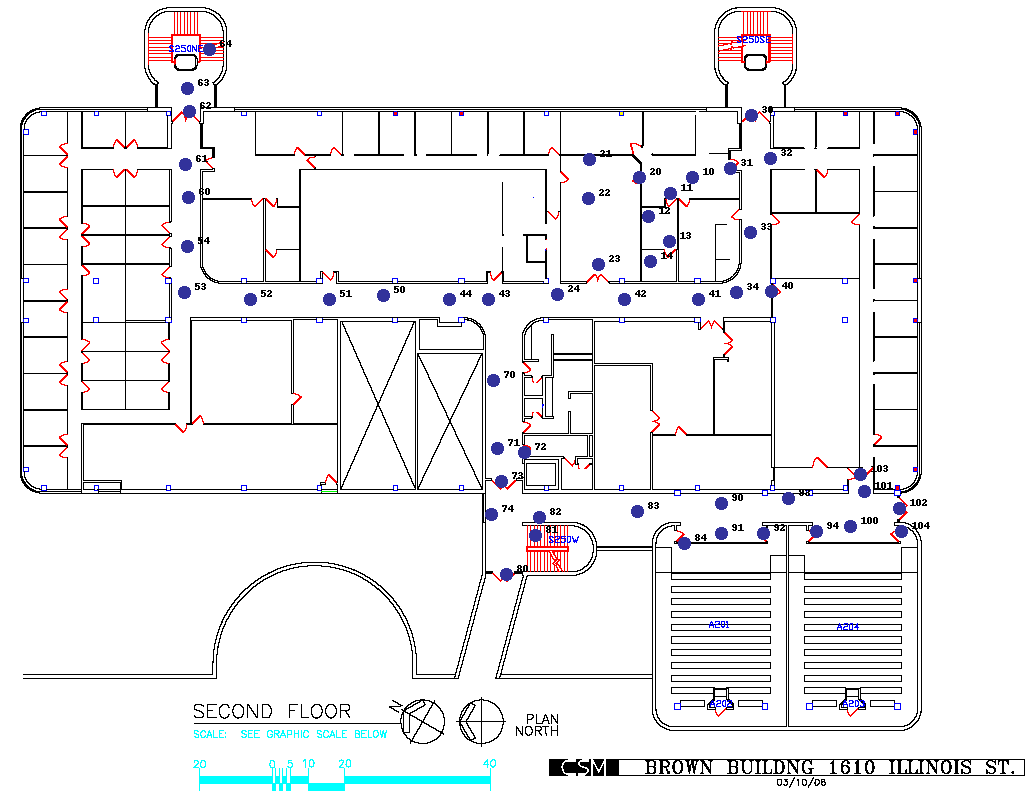
\includegraphics[width=.8\linewidth]{bb_floor2_sensors_old.png}
  \caption{Colorado School of Mines Brown building second floor.  Sensor nodes (shown as dark circles) are mounted in the ceiling of hallways and rooms.}
  \label{fig:csmbbfloor}
\end{subfigure}
\begin{subfigure}{.45\textwidth}
  \centering
  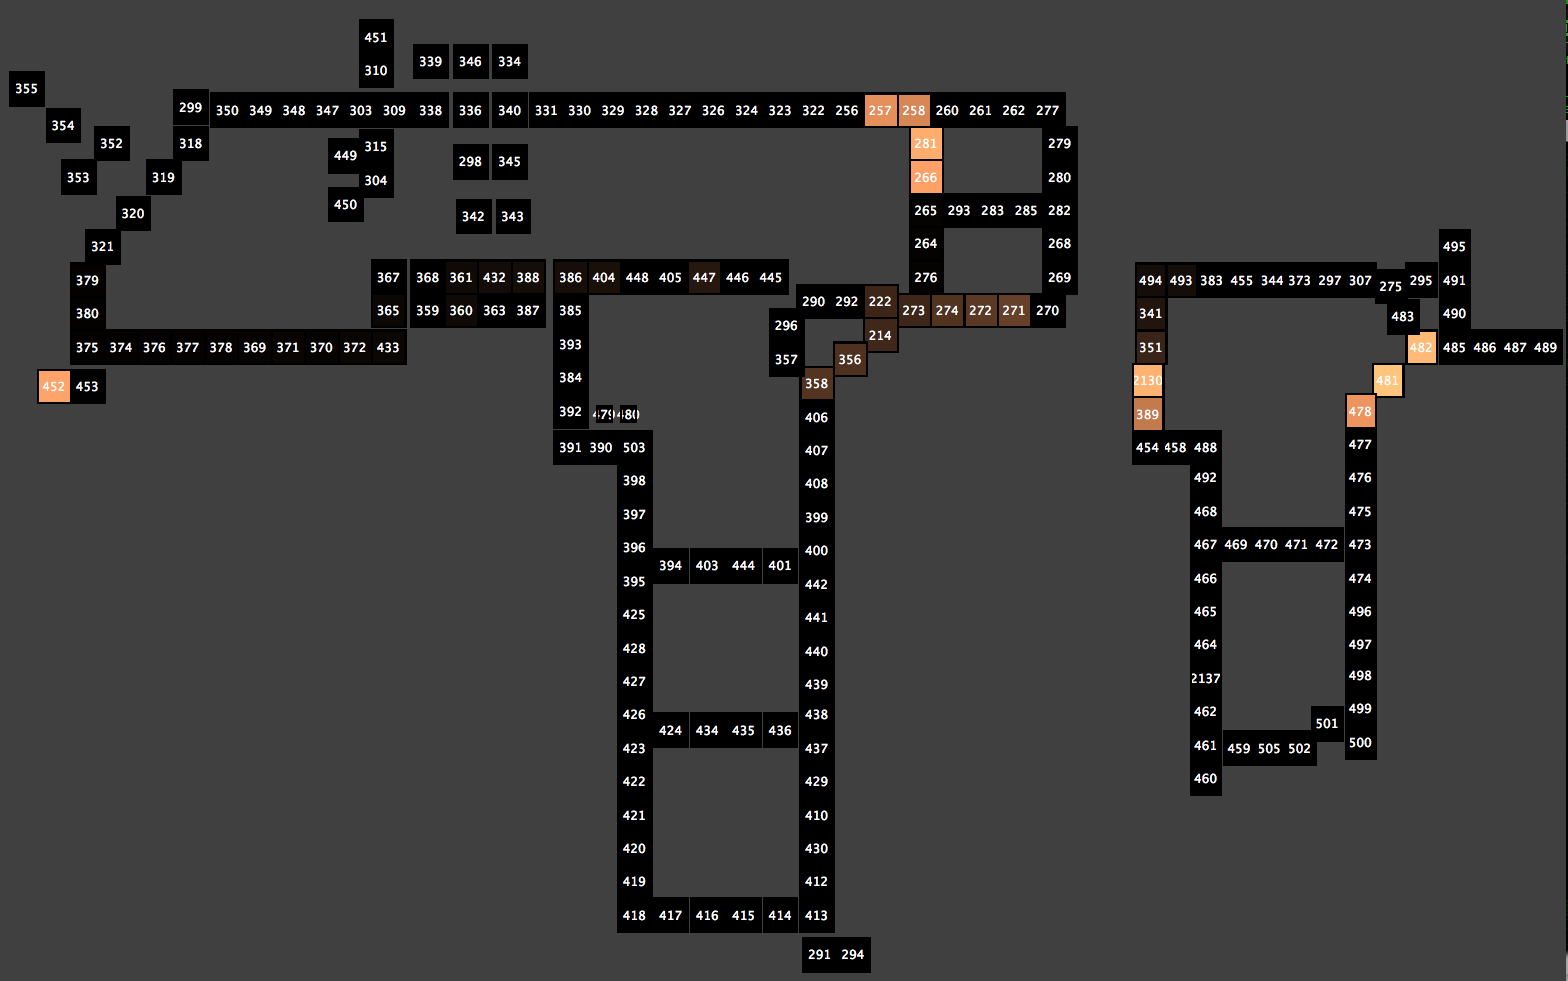
\includegraphics[width=.8\linewidth]{merl_map.png}
  \caption{MERL research lab 7th and 8th floor.  Each numbered square represents a section of hallway covered by a motion detector.}
  \label{fig:merlfloor}
\end{subfigure}
\caption{Location of IR sensors for building datasets.}
\label{fig:test}
\end{figure*}

In this work, our occupancy estimates and forecasts are derived from a set of infrared sensors that are densely placed around a building.  The data is collected from two different types of buildings.  The first data set is collected from an office building.  The other data set is collected from a classroom and research building.  We focus on short-term and medium-term forecasts; i.e., between 10 minutes to 2 hours into the future.  Although building control systems can accept forecasts up to one day into the future \cite{Ma2010}, we have found that for forecasts more than a couple of hours into the future it is better to instead rely on historic averages.  

The contributions of this paper are as follows: (1) Our work is one of the first approaches to forecasting building occupancy, as opposed to estimating the current occupancy.  (2) We have developed a modified Bayesian combined forecaster (BCF), that is capable of performing short and medium-term forecasts.  (3) We demonstrate the efficacy of the modified BCF on actual building sensor datasets, and provide insights into what forecasting algorithms will perform best under the conditions present in these buildings.  

The remainder of the paper is laid out as follows: Section 2 introduces the datasets and gives a brief description of the data collection method and the types of buildings from which the data was generated.  Section 3 discusses the details of Bayesian combined forecasting along with our modifications for improvement.  In Section 4 we briefly describe the component models used to train our Bayesian combined forecaster.  Section 5 gives a discussion of our results.  Finally Section 6 contains our conclusions.

\section{Occupancy Data}
 
Our datasets come from two sources.  The first is a combined research and office building from Mitsubishi's Electronic Research Lab (MERL) dataset \cite{Wren2007}.  The second is a classroom and office building from the Colorado School of Mines (CSMBB) \cite{Hoff2009}.  Both datasets use passive infrared sensors (Figure~\ref{fig:pirsensor}) to estimate motion in an area.  Due to the nature of IR sensors, we are only able to detect motion instead of actual occupancy; for example, a group of three people would occur as one reading in both systems.  

Despite this drawback, real occupancy data would likely be similar to our data, but with higher variance and higher means.  As the range of occupancy estimates in our two datasets are quite different and we are able to achieve accurate estimates in both scenarios, we do not foresee problems when applying our forecasting techniques to more accurate estimated values.  We thus believe this data sufficient to test our occupancy estimation algorithms.


\subsection{Colorado School of Mines Dataset}

The Colorado School of Mines dataset is a collection of 50 passive infrared sensors mounted on the ceiling of the second floor of a class and office room building.  The density of the sensor placement depends on the location within the building.  Outside the auditorium in the lower right of Figure~\ref{fig:csmbbfloor} is a dense collection of sensors placed approximately every few meters.  Throughout the rest of the building the sensors are placed roughly every 5 meters.  Data was collected for one academic school year from 2008 to 2009 and there are more than 23 million sensor readings.  To acquire readings, the sensors were polled every second and recorded data if motion was detected.  

\begin{figure}[h]
\centering
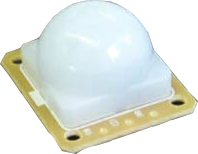
\includegraphics[width = .4\linewidth]{pir_sensor.png}
\caption{Passive infrared motion detector}
\label{fig:pirsensor}
\end{figure}

\begin{figure*}[t!]
\centering
\begin{subfigure}{.45\textwidth}
  \centering
  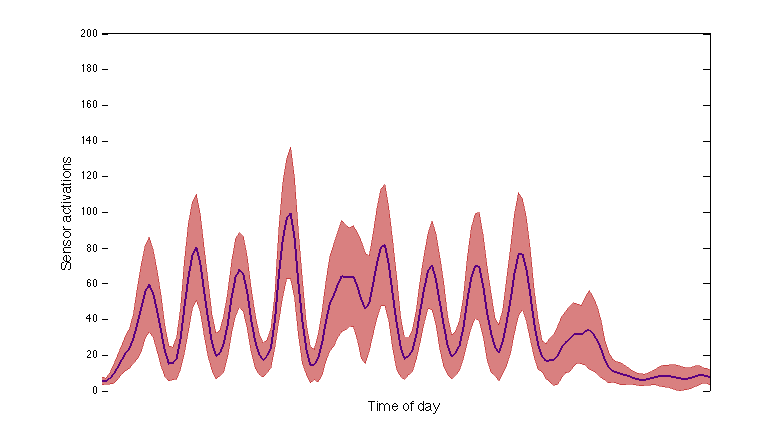
\includegraphics[width=1.0\linewidth]{brown_day.png}
  \caption{CSM Brown Building average of all Wednesdays}
  \label{fig:csmday}
\end{subfigure}
\begin{subfigure}{.45\textwidth}
  \centering
  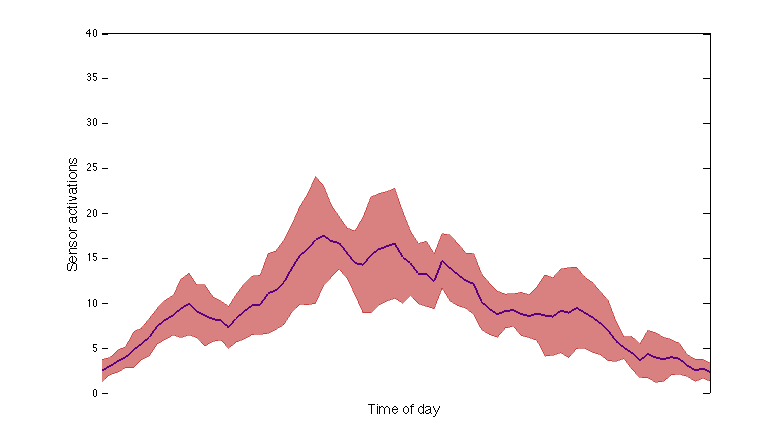
\includegraphics[width=1.0\linewidth]{merl_day.png}
  \caption{MERL average of all Wednesdays}
  \label{fig:merlday}
\end{subfigure}
\caption{Average sensor activations for a specific sensor on Wednesdays with one standard deviation range.}
\label{fig:dayplot}
\end{figure*}

This dataset is much different than the MERL dataset as classes typically provide activity on a rigid schedule during the day.  Also as students have exams and projects, late night motion is sporadic based on the time of year.  The counts of sensor activations have been aggregated over every 10 minutes.  Despite occasional late night motion during exam time, most nights have no significant motion.  For this reason we focus on data between 7:00am and 7:00pm daily.  A plot of the average activations of all Wednesdays for a single sensor along with a range of one standard deviation is given in Figure~\ref{fig:csmday}.  The defined peaks in the dataset correlate to class start and end times when most students will be in the hallways of the building.


\subsection{MERL Dataset} 

The Mitsubishi Electronic Research Labs dataset is derived from a collection of over 200 passive infrared sensors place densely throughout the 7th and 8th floor of a research office building.  The sensors are placed roughly two meters apart on the ceilings, creating a dense sensing area with little non-sensed space.  Readings are taken at the millisecond level, but due to the sensors' settling times the inter-detection time of motion is approximately 1.5 seconds.

The data was collected from March 2006 through March 2008 and there are roughly 53 million sensor readings.  This building is similar to most office buildings with a number of personal offices along with labs and conference rooms.  Employees have roughly set schedules and holidays are observed as normal. 

The counts of sensor activations have been aggregated every 10 minutes.  Because of the lack of significant motion in the night, we look only at activations that occur between 6:00am and 7:00pm daily.  A plot of the average activations of all Wednesdays for a single sensor along with a range of one standard deviation is given in Figure~\ref{fig:merlday}.  

Peak motion unsurprisingly occurs during the middle of the day corresponding to lunch time.  There is another small peak of motion near the start of the day corresponding to people entering.  Near the end of the day, instead of a peak there is a region corresponding to high variance.  This seems to imply that while people enter at roughly the same time, there is a significant variance on when people leave the building.


\section{Bayesian Combined Forecasting}
The BCF approach \cite{Petridis2001} is one of several types of methods which attempt to combine other forecasting models for time series. We selected this forecasting method over other multiple model forecasting methods (such as mixture of experts or ensembles of neural networks) due to its modularity and strong statistical backing.  BCF is modular in that it allows for the component forecasting models to come from any trained forecaster with a well defined distribution of the forecaster's mis-forecasts.  Its statistical backing comes from its direct derivation from Bayes' rule.

This section derives the BCF approach for readers unfamiliar with it and then describes some modifications of the approach which improves its performance for our application.

\subsection{Notation}
We define the time series dataset used in these models as $\{T_{t}^{(m)}\}$.  In our application the data used for these models comes from a set of $M$ binary infrared sensors.  Each $T_{t}^{m}$ is a 10 minute aggregate of the readings from sensor $m$ reading at time block $t$.  

Forecasts for a given model $k$ from the set of all models $K$ are represented by 
\begin{equation}
\bar{T}_{t + 1}^{k, m} = f(T_{t}, ..., T_{1}; \theta_{k}).
\end{equation}
\noindent
Thus the forecast of $T_{t + 1}$ is a function of all past data and some trained parameterization $\theta_{k}$ for that model. 

In this work we need to forecast more than one time step into the future.  Future forecasts are performed through iterative one step ahead forecasts.  Also for this work we forecast a model for each individual sensor and for convenience drop the $m$ from our forecasting notation.  An example of a forecast two time steps ahead of current time $t$ is given by 
\begin{equation}
\bar{T}_{t + 2}^{k} = f(\bar{T}_{t + 1}, T_{t}, ..., T_{1}; \theta_{k}).
\end{equation}
\noindent
Such a forecast is simply the forecast for one time step into the future but now with the forecasted value of $\bar{T}_{t + 1}$ used as the most recent datapoint to forecast $\bar{T}_{t + 2}$.  Forecasting in this nature allows for forecasts any number of time steps into the future. 

\begin{figure*}[t]
\centering
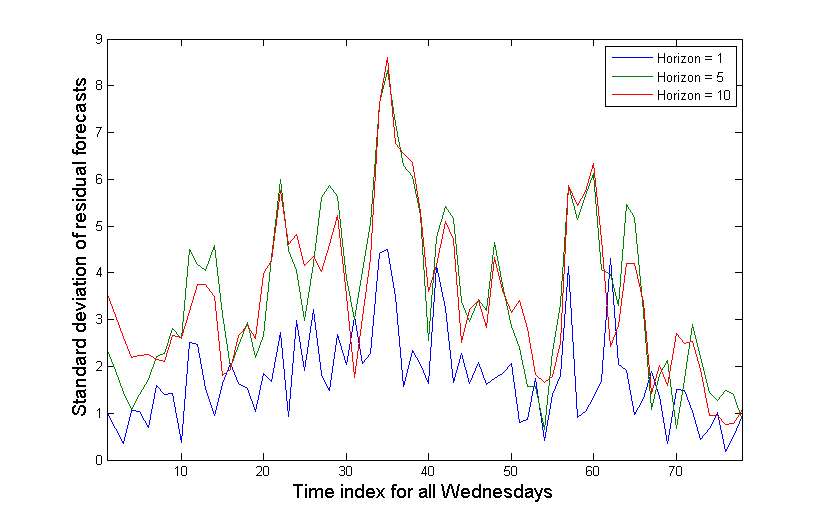
\includegraphics[width = .55\linewidth]{svm_standard_deviations_vs_horizon.png}
\caption{Standard deviation of support vector machine residuals for all Wednesdays in MERL dataset.  Time index represents 10 minute intervals from 6:00am to 7:00pm.}
\label{fig:svmstd}
\end{figure*}

\subsection{Bayesian Combined Forecasting Derivation}
To derive BCF we first assume the existence of $K$ models.  From these $K$ models, we want to create a probability distribution on a new random variable $z$ that is used to determine if model $k$ is the correct model from which to forecast at time $t$.  To do this we use the notation of Petridis \cite{Petridis2001} and define $p_{t}^{k}$ as follows
\begin{equation}
p_{t}^{k} = p(z = k | T_{t}, ..., T_{1}).
\end{equation}

From here we apply Bayes rule and get
\begin{equation}
p_{t}^{k} = \frac{p(T_{t} | z = k, T_{t - 1}, ..., T_{1}) \cdot p(z = k | T_{t - 1}, ..., T_{1})} {p(T_{t}, ..., T_{1})}.
\end{equation}
\noindent
Notice that $p(z = k | T_{t - 1}, ..., T_{1}) = p_{t - 1}^{k}$.  Thus we can create a recursive estimation based on prior $p_{t}^{k}$.

With recursive values for $p_{t}^{k}$ and replacing $p(T_{t}, ..., T_{1})$ with a conditional probability on $z$ we get
\begin{equation}
p_{t}^{k} = \frac{p(T_{t} | z = k, T_{t - 1}, ..., T_{1}) \cdot p_{t - 1}^{k}} {\sum_{j = 1}^{K}p(T_{t} | z = j, T_{t - 1}, ..., T_{1}) \cdot p_{t - 1}^{j}}.
\end{equation}

We use the empirically observed forecasting error for each model to estimate $p(T_{t}|z = k, T_{t - 1}, ..., T_{1})$.  The forecasting error for a given model at time $t$ is 
\begin{equation}
e_{t}^{k} = \bar{T}_{t}^{k} - T_{t}.
\end{equation}
\noindent
We can use these forecasting errors to estimate a probability distribution for each model on the random variable $e_{t}^{k}$.  This is typically modeled as a white noise zero mean Gaussian process.  For our work, we represent this as a distribution of error terms with some parameterization $\omega_{k}$.  Thus for each model the probability error distribution function on the model error random variable is given by $q(e_{t}^{k};\omega_{k})$.

The final equation for the posterior probability of a given model $k$ is
\begin{equation}
\label{eq:model_prob}
p_{t}^{k} = p(z = k|T_{t}, ..., T_{1}) = \frac{p_{t - 1}^{K} \cdot q(T_{t} - \bar{T}_{t}^{k}; \omega_{k})}{\sum_{j=1}^{K}p_{t - 1}^{j} \cdot q(T_{t}^{j} - \bar{T}_{t}^{j}; \omega_{j})}.
\end{equation}

An example of these changing normalized posterior probabilities for a small section of the MERL dataset is shown in Figure~\ref{fig:probsmerl}.

Forecasting using BCF is done by either computing a weighted forecast $\delta$ time steps into the future for each forecasting model or by simply selecting the model with the highest likelihood.  For this paper we forecast using a weighted forecast of all models.  The forecasting equation is
\begin{equation}
T_{t + \delta}^{ALL} = \sum_{k=1}^{K}p_{t}^{k} \cdot \bar{T}_{t + \delta}^{k}.
\end{equation}

\begin{figure}
\centering
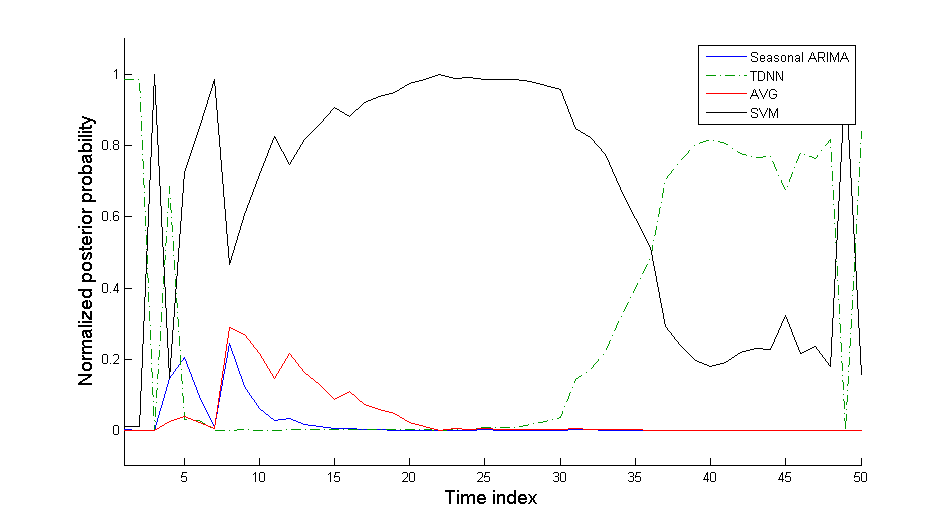
\includegraphics[width = 1.0\linewidth]{posterior_probs.png}
\caption{Normalized posterior probabilities of component models on a section of MERL dataset.}
\label{fig:probsmerl}
\end{figure}

\subsection{BCF Modifications}
In this subsection we discuss a number of modifications to maximize the effectiveness of BCF for our data.  We refer to the modified BCF algorithm as Bayesian Combined Forecasting for multiple Time Steps or BCF-TS for short.  These modifications  enable BCF to work with forecasting horizons greater than one in the future.

\subsubsection{Forecast $\delta$ time steps into the future}
Traditional implementations of BCF in other domains \cite{Petridis2001, Zheng2006} are interested only in 1 time step ahead forecasts.  For our work we require forecasts that are $\delta$ steps ahead which requires a small change to the BCF method.  Instead of generating a model's error distribution from 
\begin{equation}
e^{t}_{k} = \bar{T}_{t}^{k} - T_{t} = f(\bar{T}_{t},T_{t - 1} ..., T_{1}; \theta_{k}) - T_{t}.
\end{equation}

The error distribution is instead generated from 
\begin{equation}
e^{t}_{k} = f(\bar{T}_{t}, ..., \bar{T}_{t - \delta + 1}, T_{t - \delta}, ..., T_{1};\theta_{k}) - T_{t}.
\end{equation}
The reason for this change is due to the assumption that our error distribution is an accurate representation forecasting accuracy.  
The forecasting error distribution for models at $1$ time step into the future is not necessarily the same as models at $\delta$ time steps.  Thus we compute a different error distribution for each forecast time step.


\subsubsection{Improving model error distributions}
Despite other implementations of BCF using fixed error distributions, our data has clear daily trends.  For some of our models, the forecasted residuals follow these same trends.  See Figure~\ref{fig:svmstd} for an example of how the forecasting error distribution for a trained support vector regression model on the MERL dataset depends on the time and on the forecasting horizon.

To represent a more realistic error distribution instead of a fixed white noise Gaussian that is commonly used in the literature, we fit a Gaussian for each 10 minute slice of a given day.  The data from the MERL dataset was used from 6:00am to 7:00pm. The thirteen hours of data used per day represent 78 time slices.  For example taking the data for each time slice for each Wednesday results in 78 Gaussian error distributions for each forecasting horizon.  These Gaussians are computed from a validation set representing 20\% of our data.  It is from this set of models error distributions that we compute BCF.

As a possible improvement to this set of error distributions, we note that using a generalized autoregressive conditional heteroskedastic (GARCH) model \cite{Box2008} or some other appropriate model to forecast future variance based on local and historic changes in variance would likely outperform our time based average Gaussian models.  GARCH models are similar to seasonal autoregressive moving average models which we use as one of our component forecasting models.

\subsubsection{Model selection thresholding}
Diebold \cite{Diebold1991} cautions against the use of forecasting using a Bayesian combination of models in all cases.  Diebold points out that under certain situations a convex combination of forecasts for models may not be optimal, and cases exist where taking negative likelihood weighting may be optimal.  These conditions are likely to arise during instances where the data may not be accurately described by any of the forecasting models.  

Furthermore when such cases where no model is able to provide an accurate forecast, then it is often the case that forecasts come from the worst model.  

To combat this case, we have implemented a model selection threshold $h_{k}$.  If the likelihood of all component models is below $h_{k}$, then we forecast from only the model which is historically the most accurate based on our validation set.  

The threshold is different for each model, and should depend on the error distribution of the model.  In practice we have found that $2\sigma$ serves as a good threshold.  Basing the threshold on $\sigma$ is useful as it provides a threshold value which does not depend on $e^{k}_{t}$.  For a zero mean Gaussian the probability of the $2\sigma$ threshold is
\begin{equation}
p(2\sigma) = \frac{1}{\sigma\sqrt{2\pi}}e^{-2}.
\end{equation}
Because the Bayesian combined forecasting approach is iterative, it is possible that a long section of forecasts that indicate one model correct or incorrect can lead to likelihood underflow.  Due to this problem we adjust our normalized likelihoods so that no model may reach a value below 0.001.  This empirically chosen value is low enough to not have a great impact on forecasts while still being high enough to allow model likelihoods to change quickly.

\section{Forecasting models}
As the basis for our BCF we select from some of the most common models used for time series forecasting.  This section gives a brief introduction to each of these forecasting models. 

\subsection{Seasonal ARIMA model}
The Auto Regressive Moving Average Model (ARMA) or derivations on its form (Auto Regressive Integrated Moving Average, Seasonal Auto Regressive Moving Average, $etc$) have been used in numerous forecasting applications from economics to vehicle traffic systems.  While we have been unable to find ARMA based models used on building occupancy data directly, we have found it used to forecast building energy usage and vehicle occupancy \cite{Williams2003, Hong2011, Newsham2010}.  Its forecasting accuracy is quite strong and it can serve as a strong baseline of comparison for a forecasting problem.  

Due to that fact that our building data has periodic trends and a non stationary mean, a seasonal ARIMA model is best suited to fit our data from the class of ARMA models.  The seasonal ARIMA model is defined as:
\begin{equation}
\label{eq:sarima}
\phi_{p}(B)\Phi_{p}(B^{s})\nabla^{d}\nabla^{D}_{s}T_{t} = \theta_{q}(B)\Theta_{Q}(B^{s})e_{t}
\end{equation}
\noindent
where $\{T_{t}\}$ is our observed time series and $\{e_t\}$ represents an unobserved white noise series ($e_{t} \sim N(0, \sigma^{2})$ )the values of which are computed through model training and are not known a priori.  $B$ is the backshift operator which is a function that allows access to older time readings.  For example $BT_{t} = T_{t-1}$ and $B^{5}T_{t} = T_{t-5}$.  $\nabla^{D}_{s}$ is the seasonal difference operator ($\nabla^{D}_{s}T_{t} = (1 - B^{s})^{D}T_{t}$)and $\phi,\  \Phi,\  \theta,\ \Theta$ are trainable parameters.  

Seasonal ARIMA models are notated as
\begin{equation}
ARIMA(p,d,q)(P,D,Q)_{s}
\end{equation}
where $p$ is the number of autoregressive terms, $d$ is the number of differences and $q$ is the number of moving average terms.  $P$, $D$, and $Q$ all correspond to the seasonal equivalents of $p$, $d$, and $q$.  The parameter $s$ is the seasonality of the model.  For a full discussion of seasonal ARIMA models see Box and Jenkins \cite{Box2008}.

Finding the correct values of $p, d, q, P, D, Q, s$ is traditionally a hard problem.  To fit our parameters we use a method similar to Williams \cite{Williams2003}.  As a verification of our model, we applied the LJung-Box test \cite{Ljung1978} on our set of residual data for each model.  This tests if any of the auto correlation values on the residual dataset are significantly different from 0.  To be valid, the LJung-Box test should return a value of $p > 0.05$.  Both residual sets passed: $p = 0.9964$ for MERL and $p = 0.1072$ for CSMBB.  Our final model parameters can be seen in Table~\ref{fig:sarimatab}.  Notice that the season is different for each model due to a difference in window of time for each day that we extracted data.

\begin{table}[t]
\centering
\caption{The parameter values that were fit for MERL and CSMBB datasets for a Seasonal ARIMA model}
\begin{tabular}{|c|c|c|c|c|c|c|c|} \hline
Dataset & $p$ & $d$ & $q$ & $P$ & $D$ & $Q$ & $s$\\ \hline
MERL & 0 & 0 & 1 & 0 & 1 & 5 & 78\\ \hline
CSMBB & 0 & 1 & 1 & 0 & 1 & 3 & 72\\ \hline
\end{tabular}
\label{fig:sarimatab}
\end{table}

Forecasting from this model is performed by iteratively forward feeding values of the model into itself.  Since the set of residuals $e$ from a properly trained seasonal ARIMA model is described by a white noise Gaussian distribution $N(0, \sigma^{2})$, we can take the expected value of the residual at time $e_{t + 1}$ to be 0.  This leaves us with the following forecasting equation: 
\begin{equation}
\label{eq:sarima}
\phi_{p}(B)\Phi_{p}(B^{s})\nabla^{d}\nabla^{D}_{s}T_{t + 1} = \theta_{q - 1}(B)\Theta_{Q - 1}(B^{s})e_{t}
\end{equation}

\subsection{Historic average}
This model is simply the per day average of readings at each time step.  For certain types of data this model is has been shown to be more accurate than seasonal ARIMA forecasting \cite{Newsham2010}, specifically when the data has a strong historic correlation.  Average forecasts have the advantage of being extremely computationally fast and having a forecast accuracy that does not depend on the forecasting horizon.  This result will be shown later.

\subsection{Time delayed neural networks}

Time delayed neural networks are a special subset of regression neural networks where the input data is a local history of data from the time series.  Commonly the output is a single point forecast from that same time series at some point $t + \delta$ in the future.   The form of our 1 hidden layer time delayed neural network is:
\begin{equation}
T_{t + 1} = \phi \{ \sum_{j = 1}^{J} w_{j}\psi_{j} \bigg[ \sum_{l = 0}^{m}w_{ji}T_{t - l\delta} + w_{j0} \bigg] + w_0 \}
\end{equation}
\noindent where $\phi()$ is a linear activation function on the output layer and $\psi()$ is the standard sigmoid function.  A visual representation of the node architecture of a time delayed neural network is displayed in Figure~\ref{fig:tdnnarch}.

\begin{figure}[h]
\centering
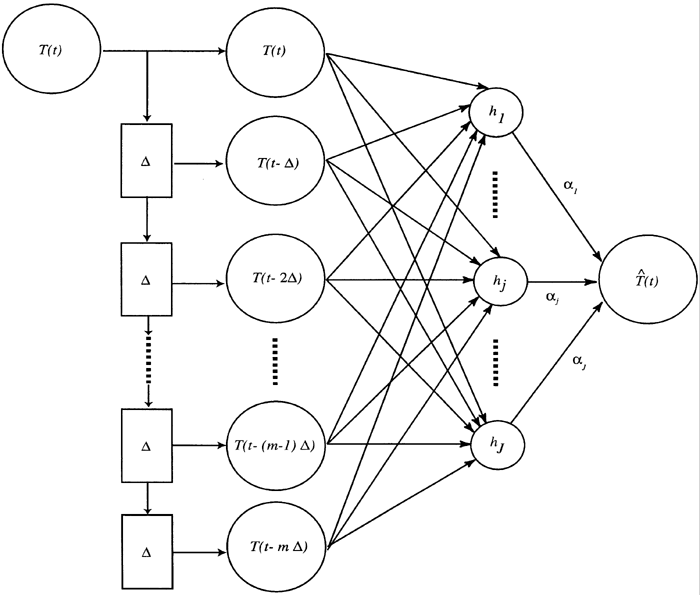
\includegraphics[width = .8\linewidth]{time_delay_neural_network.png}
\caption{Architecture of a time delayed neural network with $m + 1$ inputs and J outputs \cite{Hansen2003}.}
\label{fig:tdnnarch}
\end{figure}

Forecasting is performed by computing the output for a $m + 1$ length window of time and then iteratively forecasting a set of time steps in the future by using forecast data as inputs into the next forecast. 

The number of input nodes and hidden nodes for each dataset is given in Table~\ref{fig:tdnntab}.

\begin{table}[h]
\centering
\caption{Number of delayed input nodes and hidden nodes for MERL and CSMBB datasets}
\begin{tabular}{|c|c|c|} \hline
Dataset & Delayed input nodes & Hidden nodes\\ \hline
MERL & 15 & 8\\ \hline
CSMBB & 12 & 8\\ \hline
\end{tabular}
\label{fig:tdnntab}
\end{table}


\begin{table*}[t!]
\centering
\caption{RMSE forecast values per model for a horizon equal to one.}
\begin{tabular}{|c|c|c|c|c|c|c|} \hline
Dataset & ARIMA & TDNN & AVG & SVM & BCF & BCF-TS\\ \hline
MERL & 5.5 & 2.67 & 4.35 & 2.29 & 2.28 & \textbf{2.26}\\ \hline
CSMBB & 10.94 & 14.13 & 27.14 & 11.01 & 8.72 & \textbf{8.72}\\ \hline
\end{tabular}
\label{fig:rmsetab}
\end{table*}

\subsection{Support Vector Regression}
Support Vector Machine Regression (SVM) offers a powerful way to forecast time series.  It has been used in the past successfully to forecast travel times for vehicle traffic \cite{Wu2004}.  

As training SVM's is not done in the same way as other time series models, we first had to transform our dataset to a series of examples with a fixed window.  For a fixed window of size $w$, training input data is of the form $\{T_{t}, T_{t - 1}, ..., T_{t - w + 1}\}$.  Target data is of the form $T_{t + 1}$.  Thus the training examples which we provided to our SVM was $\{T_{t + 1}, [T_{t}, T_{t - 1}, ..., T_{t - w + 1}]\}$.

To perform SVM training we used the popular $libsvm$ package and as parameter selection is a notoriously difficult problem for SVM.  We followed the guidelines as outlined by Hsu, Chih-Chang and Lin, creators of the libsvm package \cite{Hsu2003}.  We first scaled the data by normalizing it between $[0, 1]$.  Then we searched for our best values of $C$, $\epsilon$ and $\gamma$ using the root mean squared error of the validation set a factor to determine performance of those parameters. 

For both the MERL and CSMBB datasets we used a window of 5.  This happened to be the same window length used by \cite{Wu2004}.
\section{Results}

BCF and BCF-TS (BCF with our specific set of modifications) were trained and tested using all component models described above.  All of the models were trained on 60\% of the total datasets.  Another 20\% was used for model validation and the final 20\% used for testing.  All results shown below are on the test set only.  Figure~\ref{fig:realbcf} shows an sample section of test data from the MERL dataset along with BCF-TS forecasts for horizons of 1 and 5.   As expected as the forecasting horizon increases the forecasts become less accurate.

\begin{figure}[h]
\centering
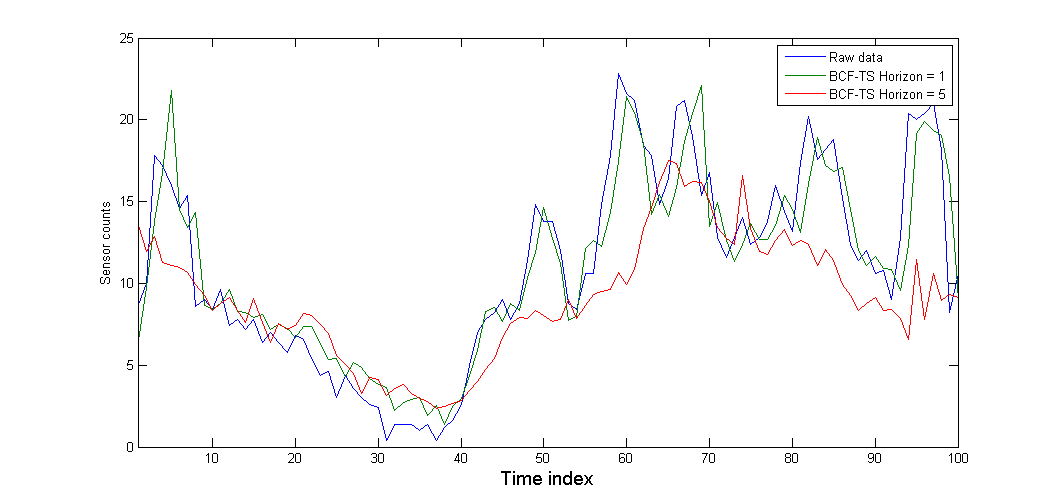
\includegraphics[width = 1.0\linewidth]{real_forecasts_bcf.png}
\caption{A comparison of forecasts at various horizons against real data for an sample time segment using BCF-TS.}
\label{fig:realbcf}
\end{figure}

It is common for one model's normalized posterior probability to be near one when that model is currently accurate.  Figure~\ref{fig:realbcfsvm} shows as example of this behavior.  From time index 1 to 8, the SVM component model has a posterior probability near 1.0 and as a result BCF-TS forecasts nearly completely from this model.  Then from time index 9 on the model's posterior probability is lower and as a result BCF-TS uses other model for its combined forecast.

\begin{figure}[h]
\centering
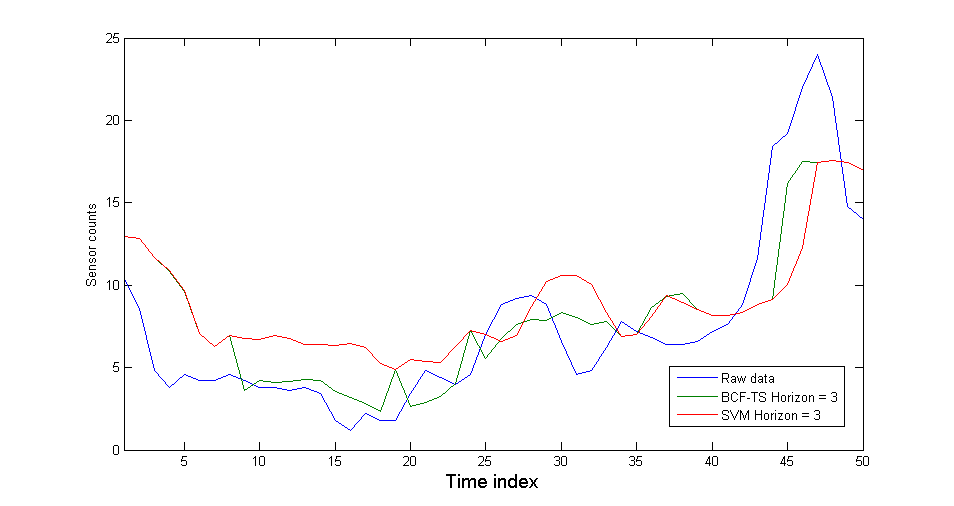
\includegraphics[width = 1.0\linewidth]{real_forecasts_bcf_svm.png}
\caption{A comparison of BCF-TS and SVM forecasts at horizon equal to three against real data.}
\label{fig:realbcfsvm}
\end{figure}

Figure~\ref{fig:rmseplot} shows the results of the root mean squared error (RMSE) of forecasts across a forecast horizon up to 10 time steps (100 minutes) into the future for each model.  These plots show that BCF-TS has the lowest error.  However, the average model shows itself to be a strong indicator of future activity for forecasts beyond 60 minutes into the future.  Forecasts were performed for significantly longer horizons, but the results were uninteresting as the total RMSE of models converged to roughly the values at a forecasting horizon of 10 time steps.  

\begin{table}
\centering
\caption{Run times (in seconds) for each forecasting horizon.}
\begin{tabular}{|c|c|c|c|c|c|c|c|} \hline
Algorithm & $1$ & $2$ & $3$ & $5$ & $8$ & $10$ \\ \hline
Average & 0.001 & 0.001 & 0.001 & 0.001 & 0.001 & 0.001 \\ \hline
ARIMA & 0.043 & 0.045 & 0.046 & 0.053 & 0.058 & 0.063\\ \hline
SVM & 0.048 & 0.910 & 0.137 & 0.227 & 0.357 & 0.444 \\ \hline
TDNN & 20.87 & 21.60 & 21.82 & 21.28 & 22.73 & 22.50 \\ \hline
BCF-TS & 20.97 & 21.26 & 21.27 & 21.34 & 21.57 & 21.63\\ \hline
\end{tabular}
\label{fig:runtimestab}
\end{table}

In the CSMBB dataset the Seasonal ARIMA model was a good forecaster of future activity while in the MERL set it performed significantly worse than even the average model on all forecasting horizons.  This is likely due to a stronger seasonal component to the CSMBB dataset due class schedules.  Instead on the MERL dataset there is little seasonal correlation and thus natural variance from a prior season may incorrectly affect current forecasts.  This result is similar to that of other papers that use seasonal ARIMA models \cite{Newsham2010}; where in the case of strong seasonal data, results are better for short horizon forecasts, but longer forecasts favor historic averages.

BCF and BCF-TS were both better at a horizon of one time step for all component models (see Table~\ref{fig:rmsetab}).  In the MERL dataset standard BCF was outperformed by SVM and later the average model for all forecast beyond one horizon.  However the BCF-TS model showed significant improvement in RMSE scores for all forecasting horizons unto 60 minutes.  For horizons of 10 time steps and greater, the average model is about as good as the BCF-TS approach.

Table~\ref{fig:runtimestab} shows the run time in seconds of each forecasting algorithm at a given forecasting horizon.  The times are for forecasting the entire test set on the MERL dataset for a single sensor, approximately twenty weeks worth of data.  In general BCF-TS was slower than any component model, but the times are still such that real-time forecasting is possible.

\begin{figure*}
\centering
\begin{subfigure}{.49\textwidth}
  \centering
  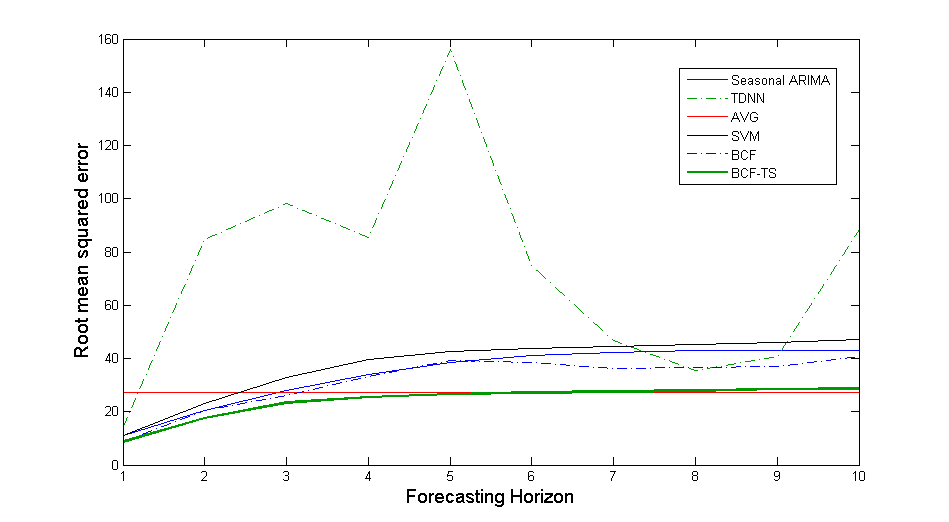
\includegraphics[width=1.0\linewidth]{brown_rmse.png}
  \caption{CSMBB forecasting model errors}
  \label{fig:csmrmse}
\end{subfigure}
\begin{subfigure}{.49\textwidth}
  \centering
  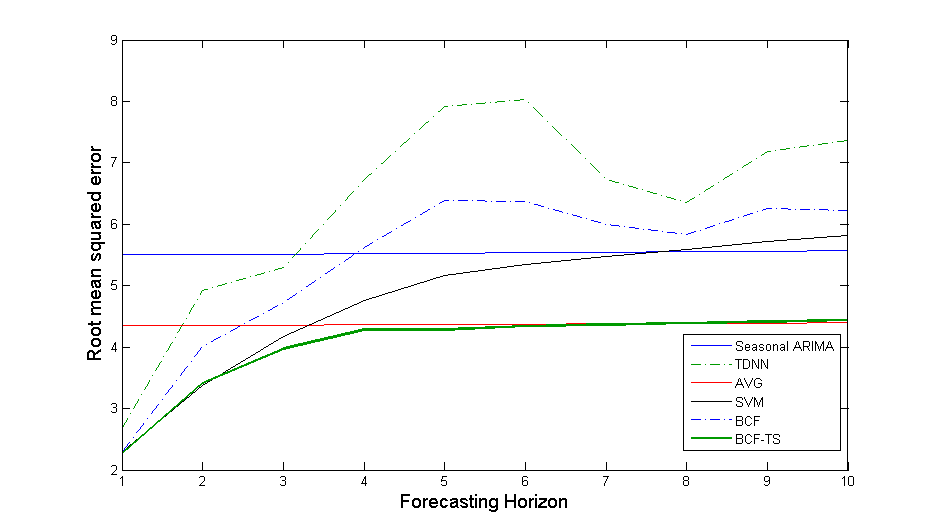
\includegraphics[width=1.0\linewidth]{merl_rmse.png}
  \caption{MERL forecasting model errors}
  \label{fig:merlrmse}
\end{subfigure}
\caption{Root mean square error of forecasting for each model vs forecasting horizon.}
\label{fig:rmseplot}
\end{figure*}

\section{Conclusion}
In conclusion, we have developed a method to forecast building occupancy from data derived from a network of simple IR motion sensors, and have applied it to two different building datasets.  Our work is novel for its application (i.e., building occupancy forecasting) and also for the Bayesian combined forecasting method that we developed to combine the results of multiple component models.  Our results show that our modified BCF approach yields more accurate forecasts than any of the component models, for short-term to medium-term forecasts.  As expected, the accuracy degrades as the forecast horizon grows longer.  For forecast horizons greater than about six time steps (corresponding to 60 minutes) into the future, the modified BCF method is no better than a simple historical daily average forecasting model.  However, even short-term forecasts of 60 minutes or less can be very useful to an intelligent building HVAC system \cite{Li2012}.

Future work could potentially improve forecasting accuracy by incorporating algorithms to more accurately predict the future error distribution for a model (we suggest using GARCH models as described in Section 3.3.2).  We also made the simplifying assumption that each sensor is independent, so that a separate model could be developed for each sensor.  However, the sensors are not independent, and it is possible that improved results could be obtained by fitting a model to a vector-valued input, consisting of the values of all sensors.  Finally, we hypothesize that occasional “anomalies” account for a significant amount of forecasting error.  By anomalies, we mean events such as snow days, cancelled classes, impromptu meetings, etc.  If these anomalies could be detected and accounted for in the models, forecasting results could be 
improved.

\section{Acknowledgements}
We acknowledge the support of the National Science Foundation (grant CNS-0931748) as well as Northrop Grumman Corp and Lockheed Martin Corp.

\bibliographystyle{abbrv}
\bibliography{big-data_mining} 
%\balancecolumns

\end{document}
